\renewcommand*{\arraystretch}{1.1}

\noindent\begin{tabularx}{17cm}{|>{\small \sf}c|X|}
	\hline
	query    & Interactive / short / 7 \\ \hline
%
	title       & Message Replies \\ \hline
%
    pattern     & \hfill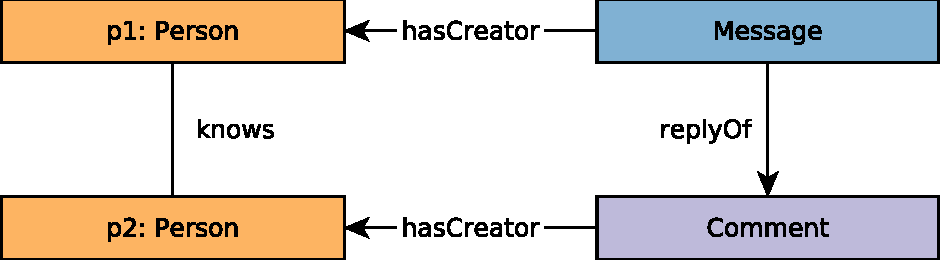
\includegraphics[scale=\patternscale,margin=0cm .2cm]{patterns/interactive-short-read-07}\hfill\vadjust{} \\ \hline
%
	desc. & Given a Message, retrieve the (1-hop) Comments that reply to it.

In addition, return a boolean flag \texttt{knows} indicating if the
author of the reply knows the author of the original message. If author
is same as original author, return false for \texttt{knows} flag.
 \\ \hline
%
	
%
	params.  &
	\vspace{1.1ex}{\begin{tabularx}{14.2cm}{|c|M|m{2cm}|Y|} \hline
	\cellcolor{parameter} \color{white} $\mathsf{1}$ & \varname{Message.id} & \cellcolor{gray!20} \vartype{ID} &  \\ \hline
	\end{tabularx}}\vspace{1.1ex} \\ \hline
%
	
	result      &
	\vspace{1.1ex}{\begin{tabularx}{14.2cm}{|c|M|m{2cm}|c|Y|} \hline
	\cellcolor{result} \color{white} $\mathsf{1}$ & \varname{Message<-replyOf-Comment.id} & \cellcolor{gray!20} \vartype{ID} &
	    \texttt{R} &
	     \\ \hline
	\cellcolor{result} \color{white} $\mathsf{2}$ & \varname{Message<-replyOf-Comment.content} & \cellcolor{gray!20} \vartype{String} &
	    \texttt{R} &
	     \\ \hline
	\cellcolor{result} \color{white} $\mathsf{3}$ & \varname{Message<-replyOf-Comment.creationDate} & \cellcolor{gray!20} \vartype{DateTime} &
	    \texttt{R} &
	     \\ \hline
	\cellcolor{result} \color{white} $\mathsf{4}$ & \varname{Comment-hasCreator->Person.id} & \cellcolor{gray!20} \vartype{ID} &
	    \texttt{R} &
	     \\ \hline
	\cellcolor{result} \color{white} $\mathsf{5}$ & \varname{Comment-hasCreator->Person.firstName} & \cellcolor{gray!20} \vartype{String} &
	    \texttt{R} &
	     \\ \hline
	\cellcolor{result} \color{white} $\mathsf{6}$ & \varname{Comment-hasCreator->Person.lastName} & \cellcolor{gray!20} \vartype{String} &
	    \texttt{R} &
	     \\ \hline
	\cellcolor{result} \color{white} $\mathsf{7}$ & \varname{knows} & \cellcolor{gray!20} \vartype{Boolean} &
	    \texttt{C} &
	    original message author knows reply author \\ \hline
	\end{tabularx}}\vspace{1.1ex} \\ \hline
	
%
	sort        &
	\vspace{1.1ex}{\begin{tabular}{|c|l|c|} \hline
	\cellcolor{sort} \color{white} $\mathsf{1}$ & \varname{Message<-replyOf-Comment.creationDate} & \cellcolor{gray!20} $\desc$ \\ \hline
	\cellcolor{sort} \color{white} $\mathsf{2}$ & \varname{Message-hasCreator->Person.id} & \cellcolor{gray!20} $\asc$ \\ \hline
	\end{tabular}}\vspace{1.1ex} \\ \hline
	%
	%
	%
    %
\end{tabularx}
\vspace{2ex}